\documentclass[12pt]{article}

\usepackage{amsmath}
\usepackage{amssymb}
\usepackage{graphicx}
\usepackage{listings}
\usepackage{xcolor}
\usepackage{geometry}
\usepackage{hyperref}
\usepackage{enumitem}
\usepackage{caption}
\usepackage{booktabs}
\usepackage{array}
\usepackage{tikz}
\usetikzlibrary{arrows.meta, positioning, calc}
\usepackage{textcomp}

\graphicspath{{./screenshots/}}
\geometry{margin=1in}
\setlength{\parindent}{0pt}
\setlength{\parskip}{6pt}
\setcounter{secnumdepth}{0}
\tolerance=1000
\emergencystretch=\maxdimen

\lstdefinestyle{code}{
    basicstyle=\ttfamily\small,
    keywordstyle=\color{blue},
    commentstyle=\color{gray},
    stringstyle=\color{orange},
    numbers=left,
    numberstyle=\tiny,
    breaklines=true,
    columns=fullflexible,
    frame=single,
    backgroundcolor=\color{gray!10}
}

\lstdefinestyle{output}{
    basicstyle=\ttfamily\small,
    breaklines=true,
    columns=fullflexible,
    frame=single,
    backgroundcolor=\color{gray!5},
    numbers=none
}

\lstset{style=code}

\begin{document}

\begin{center}
    {\LARGE \textbf{RBE 500 -- Homework 7}} \\[6pt]
    {\large Tracy Yang} \\[4pt]
    {\large \today}
\end{center}

%=============================================================
\section{Problem 1: Robot Control}

\subsection*{Part a) PD Gain Design}

Plant: $J\ddot{\theta} + B\dot{\theta} = u$, with $J=2$, $B=0.4$.

PD control law (error $e=\theta_r-\theta$):
\[
u = K_p e - K_d \dot{\theta}.
\]

Closed loop:
\[
J\ddot{\theta} + (B+K_d)\dot{\theta} + K_p\theta = K_p\theta_r
\quad\Rightarrow\quad
\ddot{\theta} + 2\zeta\omega_n\dot{\theta} + \omega_n^2\theta = \omega_n^2\theta_r,
\]
\[
2\zeta\omega_n = \frac{B+K_d}{J}, \qquad \omega_n^2 = \frac{K_p}{J}.
\]

Design specs: critically damped ($\zeta=1$), $t_s = 4/\omega_n = 1$ s, so $\omega_n = 4$ rad/s.

\[
K_p = J\omega_n^2 = 2(4)^2 = \mathbf{32}, \qquad
K_d = 2\zeta\omega_n J - B = 2(1)(4)(2)-0.4 = \mathbf{15.6}
\]

\[
\boxed{K_p = 32, \qquad K_d = 15.6}
\]

\subsection*{Part b) Simulink Implementation}

\begin{center}
    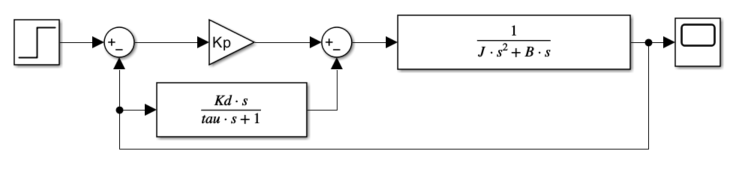
\includegraphics[width=0.75\textwidth]{closed_loop_block_diagram.png}
    \captionof{figure}{Closed-loop block diagram in Simulink (Problem 1).}
\end{center}

\textbf{Parameter script} (\texttt{params.m}):

\begin{lstlisting}
J   = 2;      % link inertia
B   = 0.4;    % effective damping
Kp  = 32;     % proportional gain
Kd  = 15.6;   % derivative gain
tau = 0.0001; % derivative filter time constant
\end{lstlisting}

\textbf{Build notes:}
\begin{itemize}
    \item \textbf{Plant.} $J\ddot\theta+B\dot\theta=u$ transforms to
          $\Theta(s)/U(s) = 1/(Js^2+Bs)$, torque to \emph{position}, not velocity, so the plant
          has a free integrator. Transfer Fcn block: Numerator \texttt{[1]}, Denominator
          \texttt{[J B 0]}. The trailing zero is required; \texttt{[J B]} alone gives torque to
          angular \emph{velocity} instead of position.
    \item \textbf{Derivative term.} An ideal \textit{Derivative} block on the error $e$ fails two
          ways: it differentiates the Step block's jump at $t=0$ (infinite slope, solver crashes),
          and it creates an \textbf{algebraic loop} with the plant, since both $u$ and $\dot\theta$
          become instantaneous functions of each other. The fix is a \textit{filtered derivative}: a
          second Transfer Fcn block realizing $\dfrac{K_d s}{\tau s+1}$ (Numerator \texttt{[Kd 0]},
          Denominator \texttt{[tau 1]}), tapped off the plant output $\theta$ rather than the error.
          This block has its own internal state, so it cannot form an algebraic loop, and it rolls
          off at high frequency instead of differentiating a discontinuity exactly. It is the same
          technique Simulink's built-in PID block uses internally.
\end{itemize}

\textbf{Numerical verification.} To avoid misreading settling time and overshoot off the scope, the
closed-loop response was also computed directly from the transfer functions:

\begin{lstlisting}
J = 2; B = 0.4; Kp = 32; Kd = 15.6; tau = 0.0001;

P = tf(1, [J B 0]);          P.InputName  = 'u';     P.OutputName = 'theta';
Dfilt = tf([Kd 0], [tau 1]); Dfilt.InputName = 'theta'; Dfilt.OutputName = 'ud';
Kp_tf = tf(Kp, 1);           Kp_tf.InputName = 'e';   Kp_tf.OutputName = 'up';

sum1 = sumblk('e = xr - theta');
sum2 = sumblk('u = up - ud');
CL = connect(P, Dfilt, Kp_tf, sum1, sum2, 'xr', 'theta');

t = 0:0.0001:3;
y = step(CL, t);
info = stepinfo(y, t)
\end{lstlisting}

\begin{lstlisting}[style=output]
info =

  struct with fields:

         RiseTime: 0.8394
    TransientTime: 1.4579
     SettlingTime: 1.4579
      SettlingMin: 0.9000
      SettlingMax: 0.9999
        Overshoot: 0
       Undershoot: 0
             Peak: 0.9999
         PeakTime: 3
\end{lstlisting}

$t_s \approx 1.46$ s with $0\%$ overshoot, slower than the 1 s target. This is addressed in Part c.

\begin{center}
    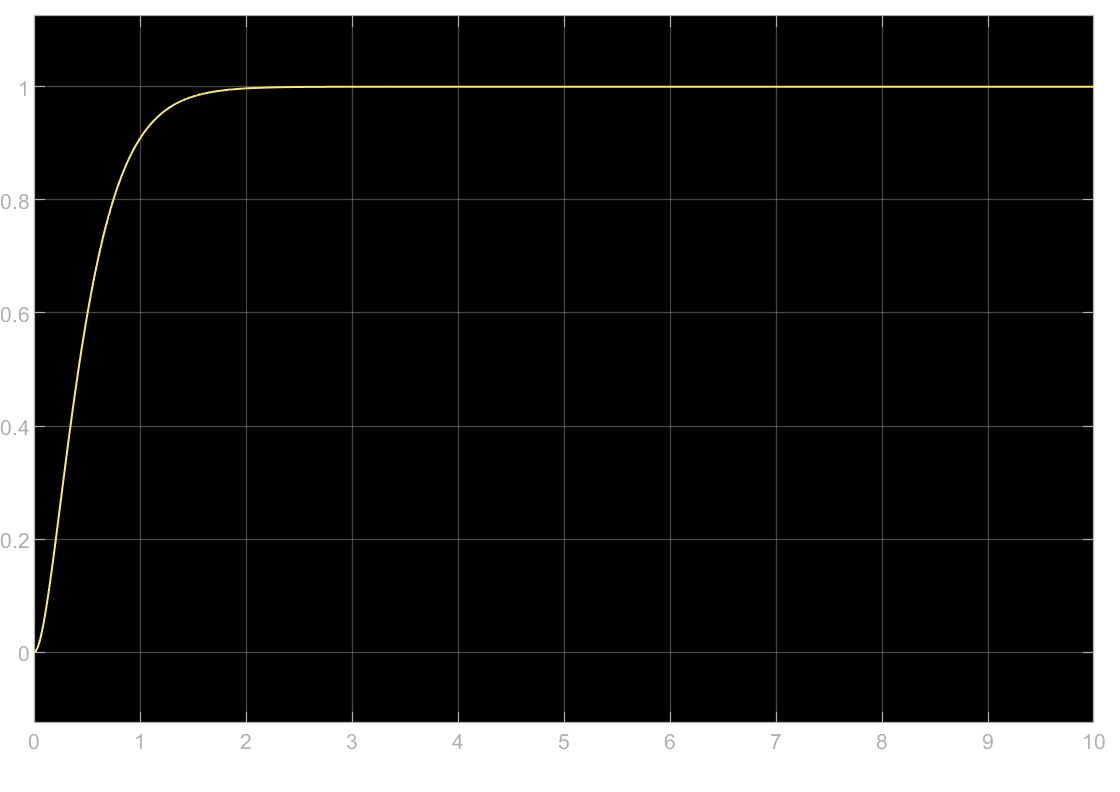
\includegraphics[width=0.75\textwidth]{initial_response_output.png}
    \captionof{figure}{Step response, $K_p=32$, $K_d=15.6$.}
\end{center}

\subsection*{Part c) Tuning}

\textbf{Why $t_s$ exceeds 1 s.} The formula $t_s=4/(\zeta\omega_n)$ comes from the decaying
exponential envelope of an underdamped response. The exact critically-damped response is
\[
\theta(t) = 1-(1+\omega_n t)e^{-\omega_n t},
\]
which decays slower than the plain exponential envelope, so at $\zeta=1$ the formula
underestimates $t_s$. This matches the measured 1.46 s versus the 1 s target.

\textbf{A modeling bug found along the way.} A mismatch between Simulink and MATLAB results
(predicted $t_s\approx0.4$ s, observed $t_s\approx3$ s) was traced by setting $K_d=0$: the resulting
slow, lightly-damped oscillation confirmed the controller logic was correct but pointed at the
plant. The Transfer Fcn had been entered as \texttt{[J B]}, missing the free integrator; correcting
it to \texttt{[J B 0]} resolved the mismatch.

\textbf{Retuning.} Requiring $(1+\omega_n)e^{-\omega_n}\le0.02$ for $t_s=1$ s gives
$\omega_n\gtrsim6$ numerically; $\omega_n=6.5$ was used for margin:

\[
K_p = J\omega_n^2 = 2(6.5)^2 = 84.5, \qquad K_d = 2\omega_n J - B = 2(6.5)(2)-0.4 = 25.6
\]

\begin{lstlisting}
J = 2; B = 0.4; Kp = 84.5; Kd = 25.6; tau = 0.0001;
% same connect() structure as above
t = 0:0.0001:3;
y = step(CL, t);
info = stepinfo(y, t)
\end{lstlisting}

\begin{lstlisting}[style=output]
info =

  struct with fields:

         RiseTime: 0.5168
    TransientTime: 0.8981
     SettlingTime: 0.8981
      SettlingMin: 0.9000
      SettlingMax: 1.0000
        Overshoot: 0
       Undershoot: 0
             Peak: 1.0000
         PeakTime: 3
\end{lstlisting}

\[
\boxed{K_p = 84.5, \qquad K_d = 25.6, \qquad \tau = 0.0001, \qquad t_s \approx 0.898\text{ s}}
\]

\begin{center}
    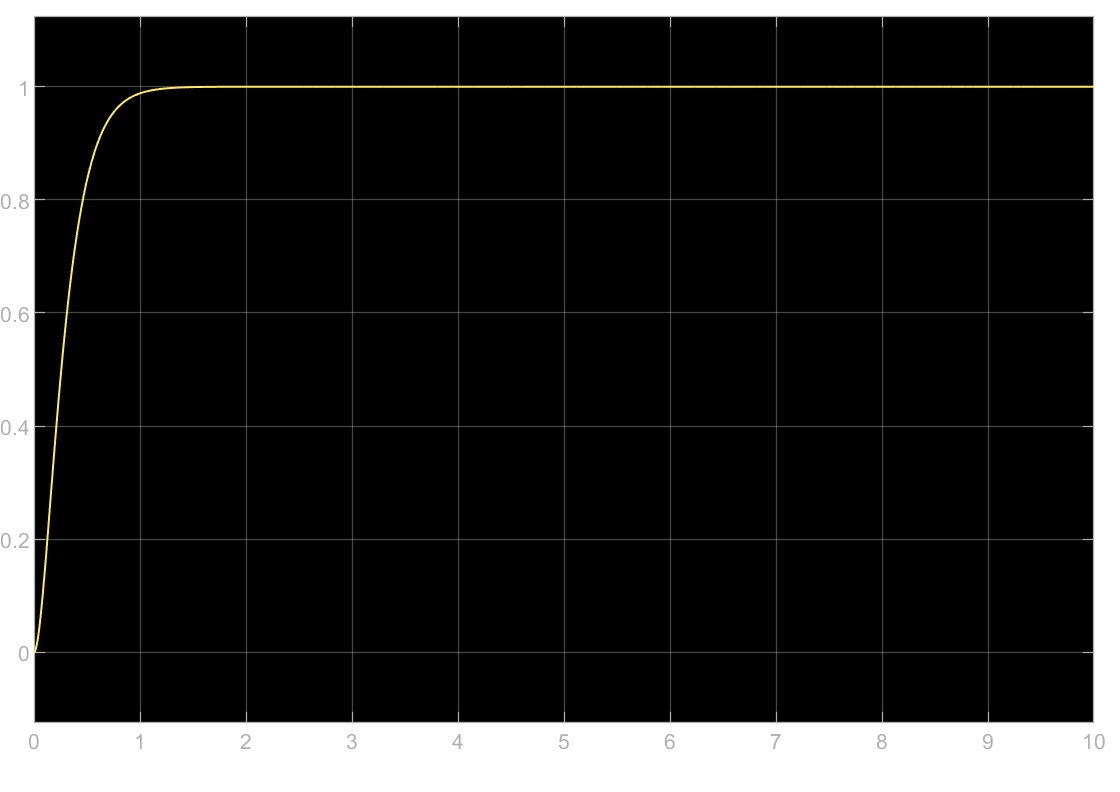
\includegraphics[width=0.75\textwidth]{tuned_response_output.png}
    \captionof{figure}{Step response after tuning.}
\end{center}

%=============================================================
\section{Problem 2: Robot Control}

System: $m\ddot{x}+b\dot{x}+kx=F$, with $m=1$, $k=1$, $b=0.5$.

PD law: $F = K_p(x_r-x) - K_d\dot x$.

Closed loop:
\[
m\ddot x + (b+K_d)\dot x + (k+K_p)x = K_p x_r
\;\Rightarrow\;
2\zeta\omega_n = b+K_d, \qquad \omega_n^2 = k+K_p.
\]

Design specs: $t_s=2$ s, no overshoot ($\zeta=1$), so $\omega_n = 4/2 = 2$ rad/s.

\[
K_p = \omega_n^2-k = 4-1 = 3, \qquad K_d = 2\omega_n-b = 4-0.5 = 3.5
\]

\[
K_p = 3, \qquad K_d = 3.5 \quad \text{(initial design; corrected below)}
\]

This plant already has a restoring term $k$, so $1/(ms^2+bs+k)$ is genuinely second order. Transfer
Fcn: Numerator \texttt{[1]}, Denominator \texttt{[m b k]}, with no trailing zero needed.

\subsection*{Steady-State Error}

Checking $K_p=3$, $K_d=3.5$ numerically:

\begin{lstlisting}
m = 1; k = 1; b = 0.5; Kp = 3; Kd = 3.5; tau = 0.0001;

P = tf(1, [m b k]);          P.InputName  = 'F';   P.OutputName = 'x';
Dfilt = tf([Kd 0], [tau 1]); Dfilt.InputName = 'x'; Dfilt.OutputName = 'ud';
Kp_tf = tf(Kp, 1);           Kp_tf.InputName = 'e'; Kp_tf.OutputName = 'up';

sum1 = sumblk('e = xr - x');
sum2 = sumblk('F = up - ud');
CL = connect(P, Dfilt, Kp_tf, sum1, sum2, 'xr', 'x');

t = 0:0.0001:5;
y = step(CL, t);
info = stepinfo(y, t)
\end{lstlisting}

\begin{lstlisting}[style=output]
info =

  struct with fields:

         RiseTime: 1.6763
    TransientTime: 2.9032
     SettlingTime: 2.9032
      SettlingMin: 0.6747
      SettlingMax: 0.7496
        Overshoot: 0
       Undershoot: 0
             Peak: 0.7496
         PeakTime: 5
\end{lstlisting}

\begin{center}
    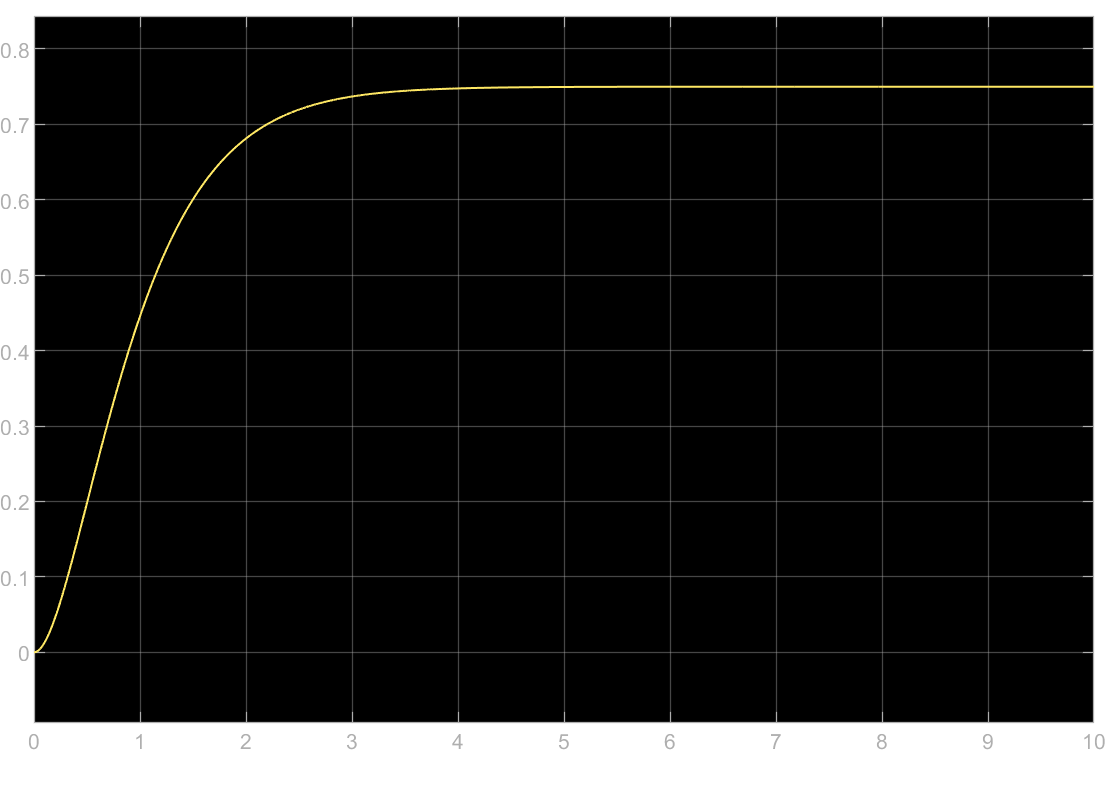
\includegraphics[width=0.75\textwidth]{steady_state_error.png}
    \captionof{figure}{Step response with $K_p=3$, $K_d=3.5$, no reference scaling. The output
    settles at 0.75, not 1.}
\end{center}

The output settles at 0.75, not 1. At steady state ($\dot x=\ddot x=0$), the closed-loop equation
gives
\[
x_{ss} = \frac{K_p}{k+K_p}\,x_r = \frac{3}{4} = 0.75.
\]
The spring constantly pulls the mass back toward $x=0$, and pure P control only balances it
proportionally; it never fully cancels the spring's restoring force. Problem 1 had no such term, so
its steady-state gain was always exactly 1.

\textbf{Fix: reference scaling.} A gain $N$ is inserted between the Step block and the first Sum
block:
\[
N = \frac{k+K_p}{K_p} \quad\Rightarrow\quad x_{ss} = \frac{K_p}{k+K_p}(N x_r) = x_r.
\]

\begin{center}
    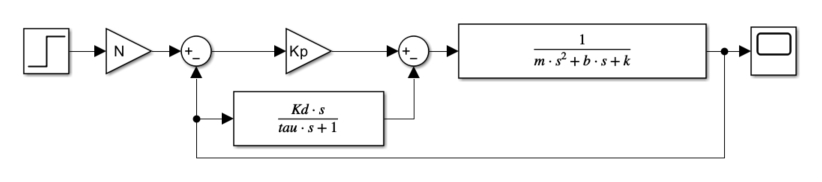
\includegraphics[width=0.75\textwidth]{closed_loop_block_diagram_2.png}
    \captionof{figure}{Closed-loop block diagram in Simulink (Problem 2), with reference-scaling
    gain $N$.}
\end{center}

\subsection*{Retuning}

With $N$ added, $K_p=3$, $K_d=3.5$ gives $t_s\approx2.90$ s, still past the 2 s target for the same
reason discussed in Part 1c. Requiring $\omega_n t_s\gtrsim6$ for a 2 s target gives $\omega_n\gtrsim3$;
$\omega_n=3.5$ was used for margin:

\[
K_p = \omega_n^2-k = (3.5)^2-1 = 11.25, \qquad K_d = 2\omega_n-b = 7-0.5 = 6.5, \qquad
N = \frac{k+K_p}{K_p} = 1.0889
\]

\begin{lstlisting}
m = 1; k = 1; b = 0.5; Kp = 11.25; Kd = 6.5; tau = 0.0001;
N = (k + Kp) / Kp;

P = tf(1, [m b k]);          P.InputName  = 'F';   P.OutputName = 'x';
Dfilt = tf([Kd 0], [tau 1]); Dfilt.InputName = 'x'; Dfilt.OutputName = 'ud';
Kp_tf = tf(Kp, 1);           Kp_tf.InputName = 'e'; Kp_tf.OutputName = 'up';
Nref = tf(N, 1);             Nref.InputName = 'xr'; Nref.OutputName = 'xr_scaled';

sum1 = sumblk('e = xr_scaled - x');
sum2 = sumblk('F = up - ud');
CL = connect(P, Dfilt, Kp_tf, Nref, sum1, sum2, 'xr', 'x');

t = 0:0.0001:5;
y = step(CL, t);
info = stepinfo(y, t)
\end{lstlisting}

\begin{lstlisting}[style=output]
info =

  struct with fields:

         RiseTime: 0.9595
    TransientTime: 1.6673
     SettlingTime: 1.6673
      SettlingMin: 0.9000
      SettlingMax: 1.0000
        Overshoot: 0
       Undershoot: 0
             Peak: 1.0000
         PeakTime: 5
\end{lstlisting}

\[
\boxed{K_p = 11.25, \qquad K_d = 6.5, \qquad N = 1.0889, \qquad t_s \approx 1.667\text{ s}}
\]

Settles exactly at $x=1$, inside the 2 s target, with $0\%$ overshoot.

\textbf{Parameter script} (\texttt{params2.m}):

\begin{lstlisting}
m   = 1;         % mass
k   = 1;         % spring constant
b   = 0.5;       % damping coefficient
Kp  = 11.25;     % proportional gain
Kd  = 6.5;       % derivative gain
N   = (k+Kp)/Kp; % reference scaling
tau = 0.0001;    % derivative filter time constant
\end{lstlisting}

\begin{center}
    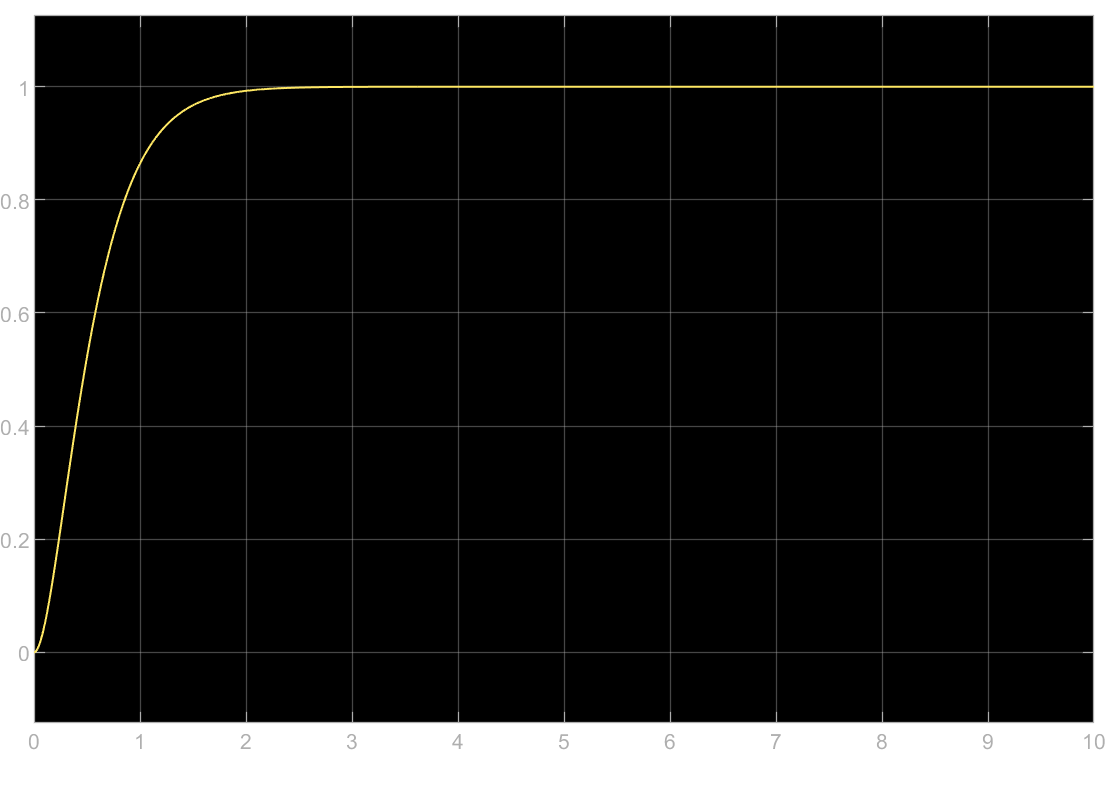
\includegraphics[width=0.75\textwidth]{tuned_response_output_2.png}
    \captionof{figure}{Step response, $K_p=11.25$, $K_d=6.5$, $N=1.0889$.}
\end{center}

\end{document}